\chapter{User Interface Design}

\section{Navigation Overview}
In this section we are going to present the whole navigation structure of CookingTime application, the starting decision was to make a simple structure of application screen in order to let users finding all the requirede screen in few tap as presentend in the picture below.
\begin{figure}[H]
	\centering
	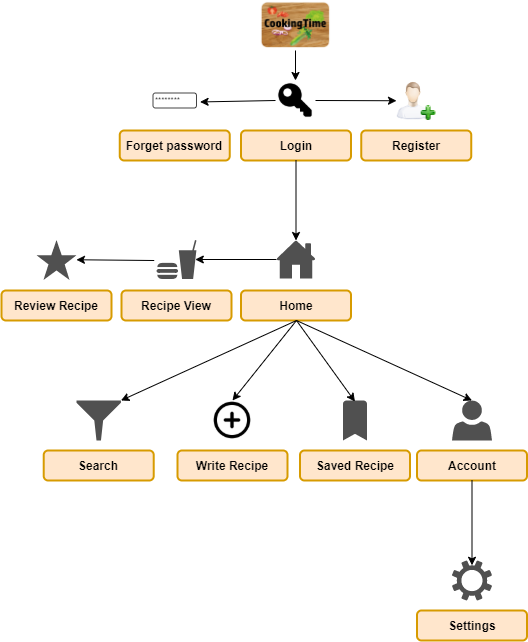
\includegraphics[width = .5\linewidth]{img/CookingTimeNavigator.png}
	\caption{App Navigation Structure}
\end{figure}

\section{Mockup screens}
In the following section there are some mockups of the application together with the explanation of all the feature reachable by the represented screen.

\subsection{Log In}
\begin{figure}[H]
	\centering
	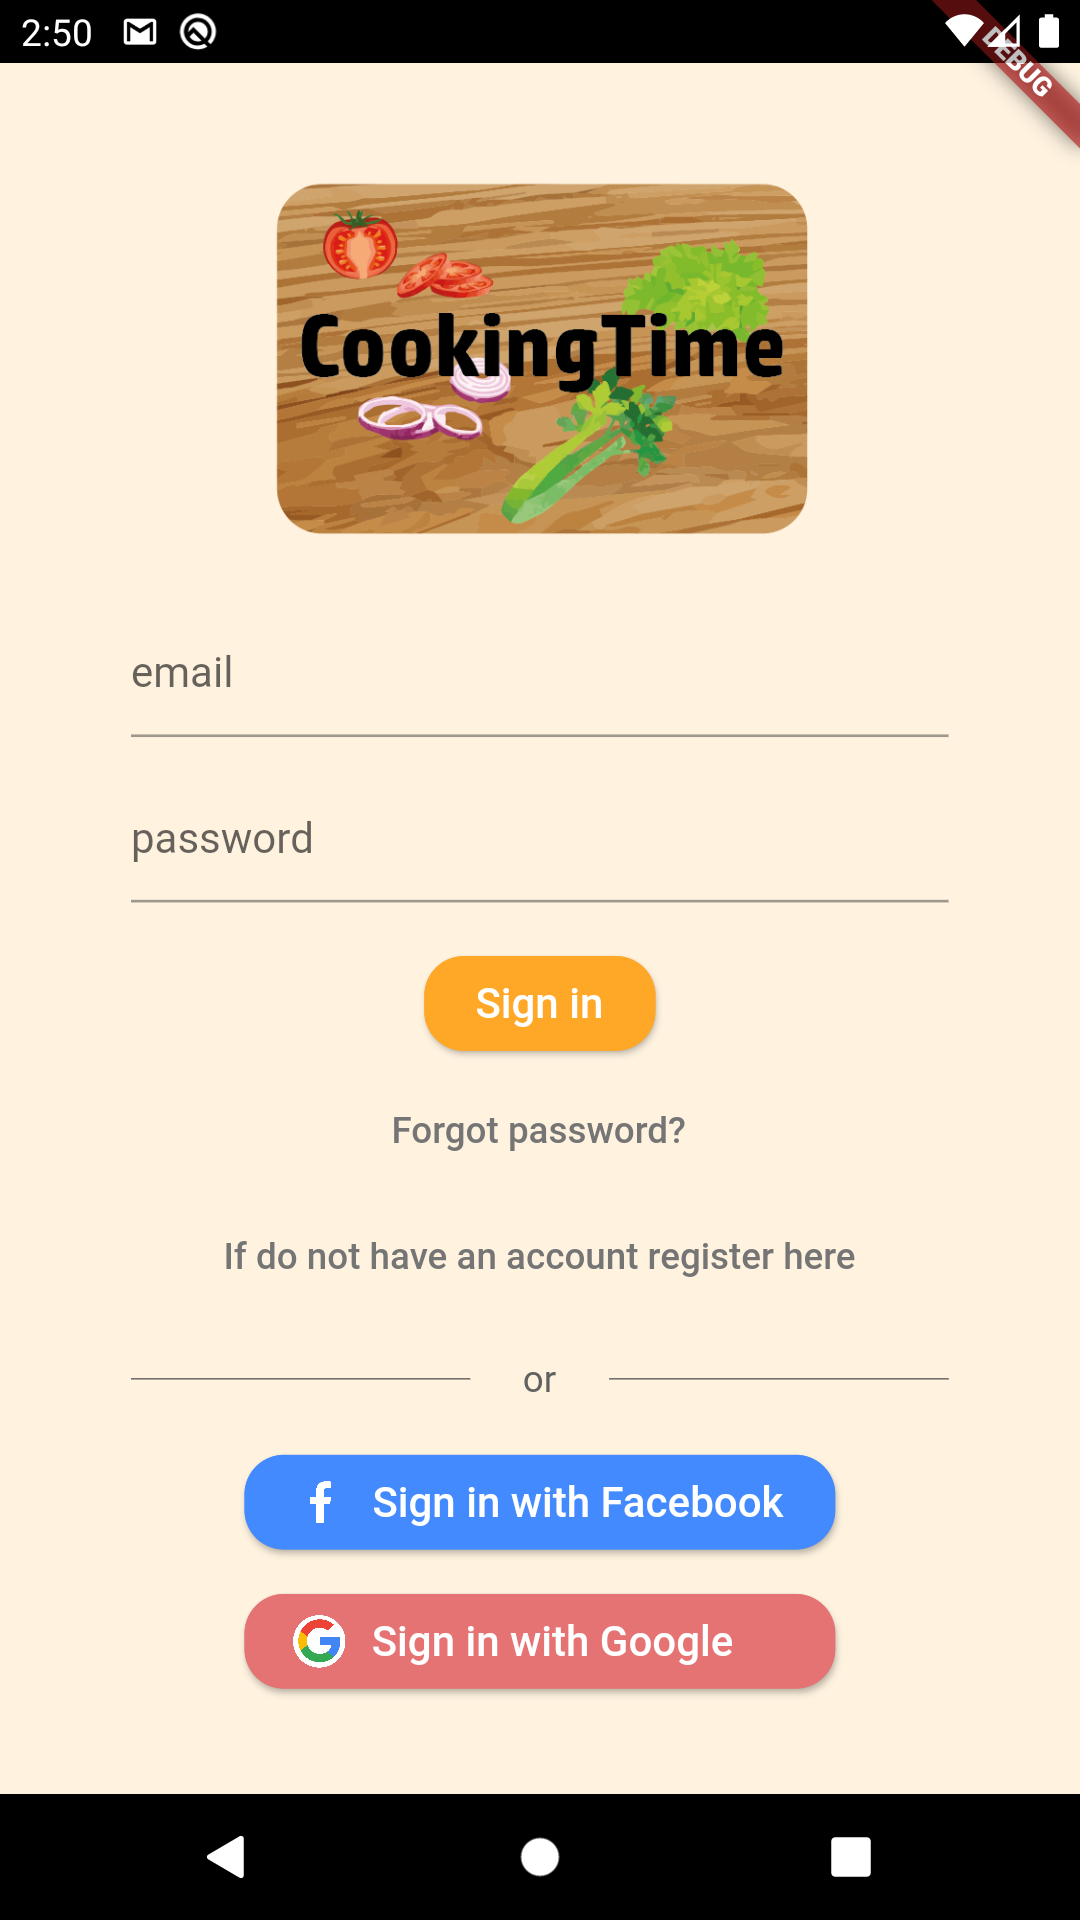
\includegraphics[width = .3\linewidth]{img/SignIn.png}
	\caption{Login Screen}
\end{figure}
This is the first screen which the user sees after the opening of the application, here he can login using his credentials, moreover he can go to the registration page or the lost password page.

\subsection{Registration}
\begin{figure}[H]
	\centering
	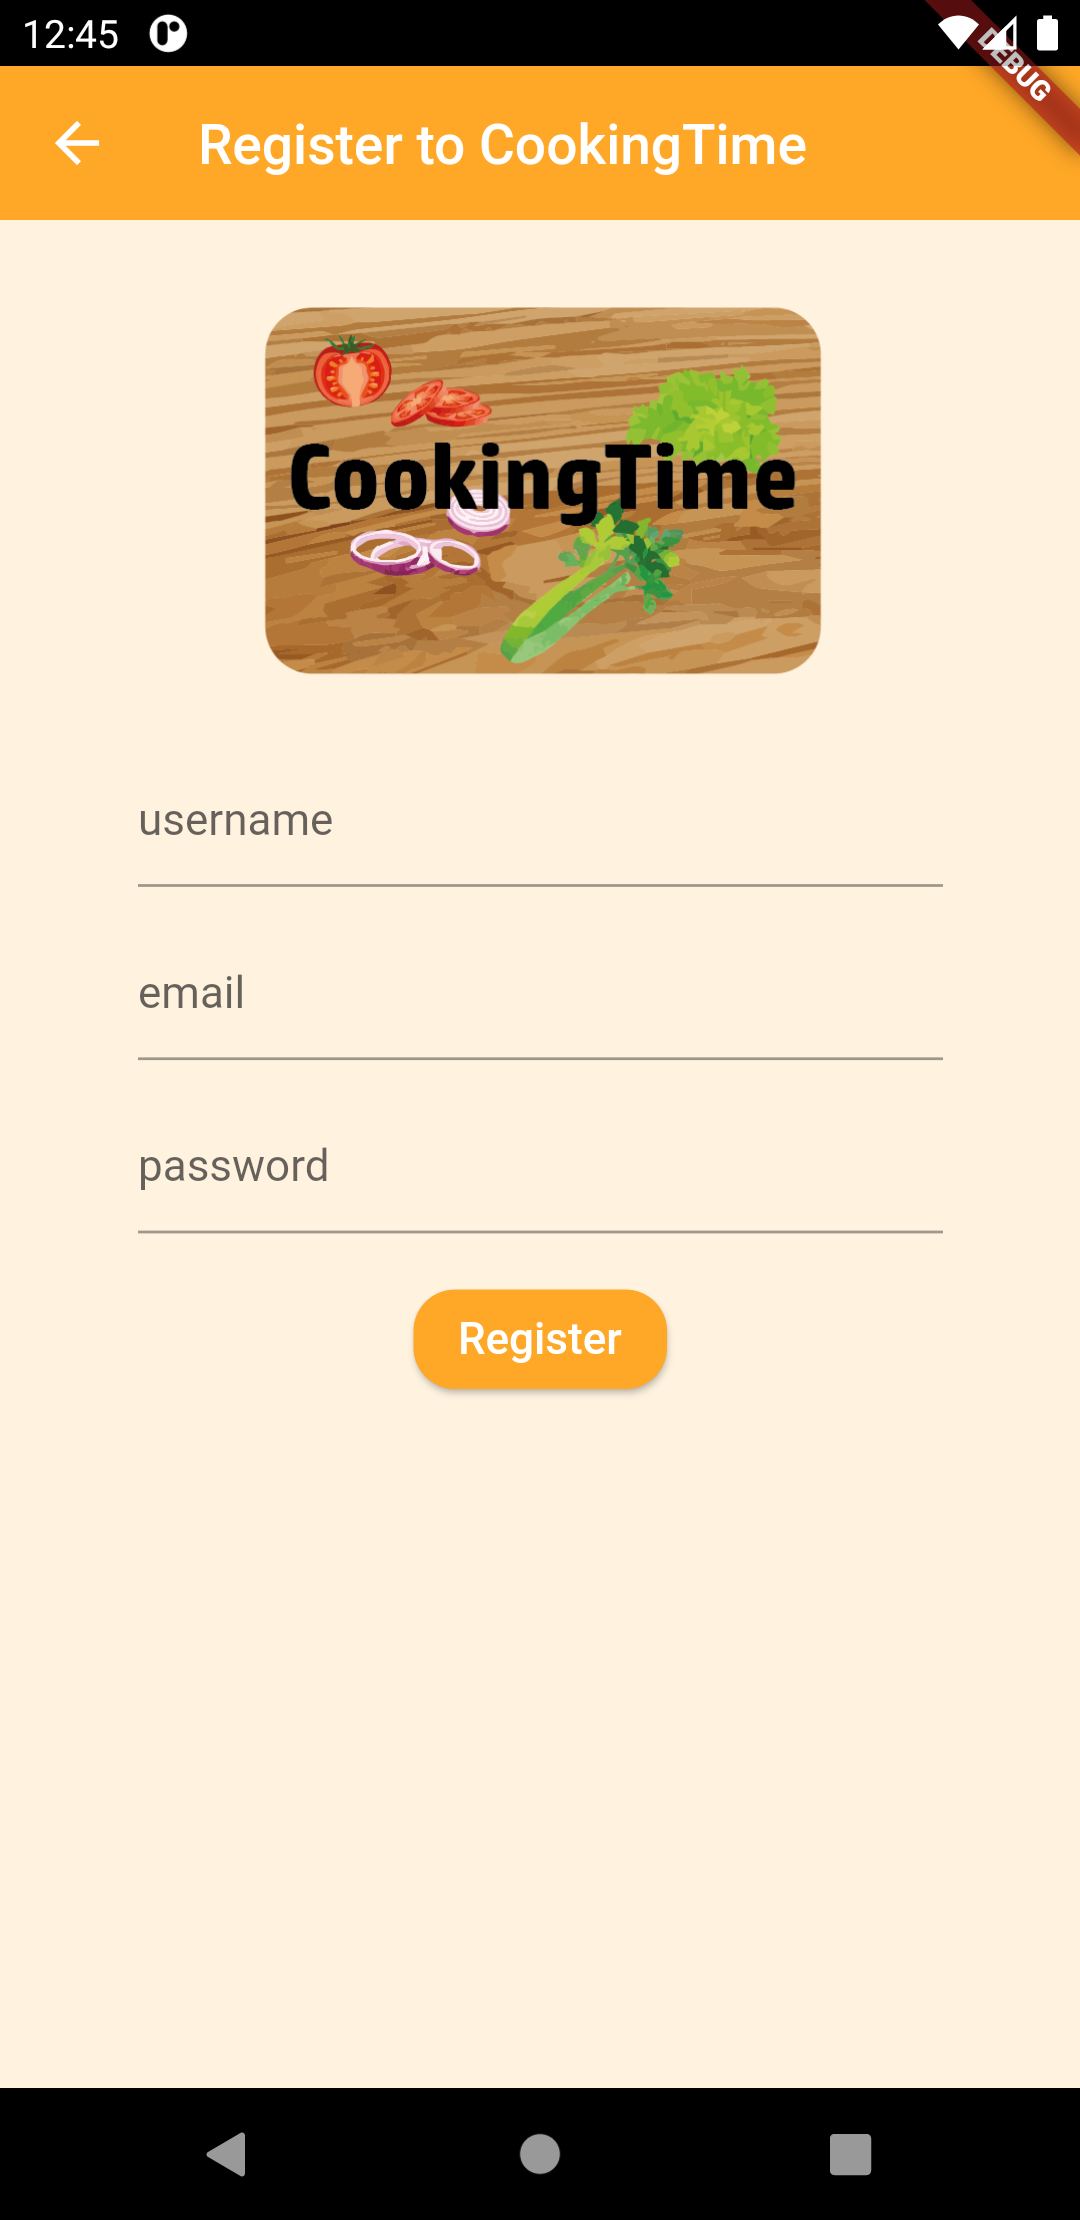
\includegraphics[width = .3\linewidth]{img/Registration.png}
	\caption{Registration Screen}
\end{figure}
This screen allows the user to register in the application providing a username, email and password.

\subsection{Password Reset}
\begin{figure}[H]
	\centering
	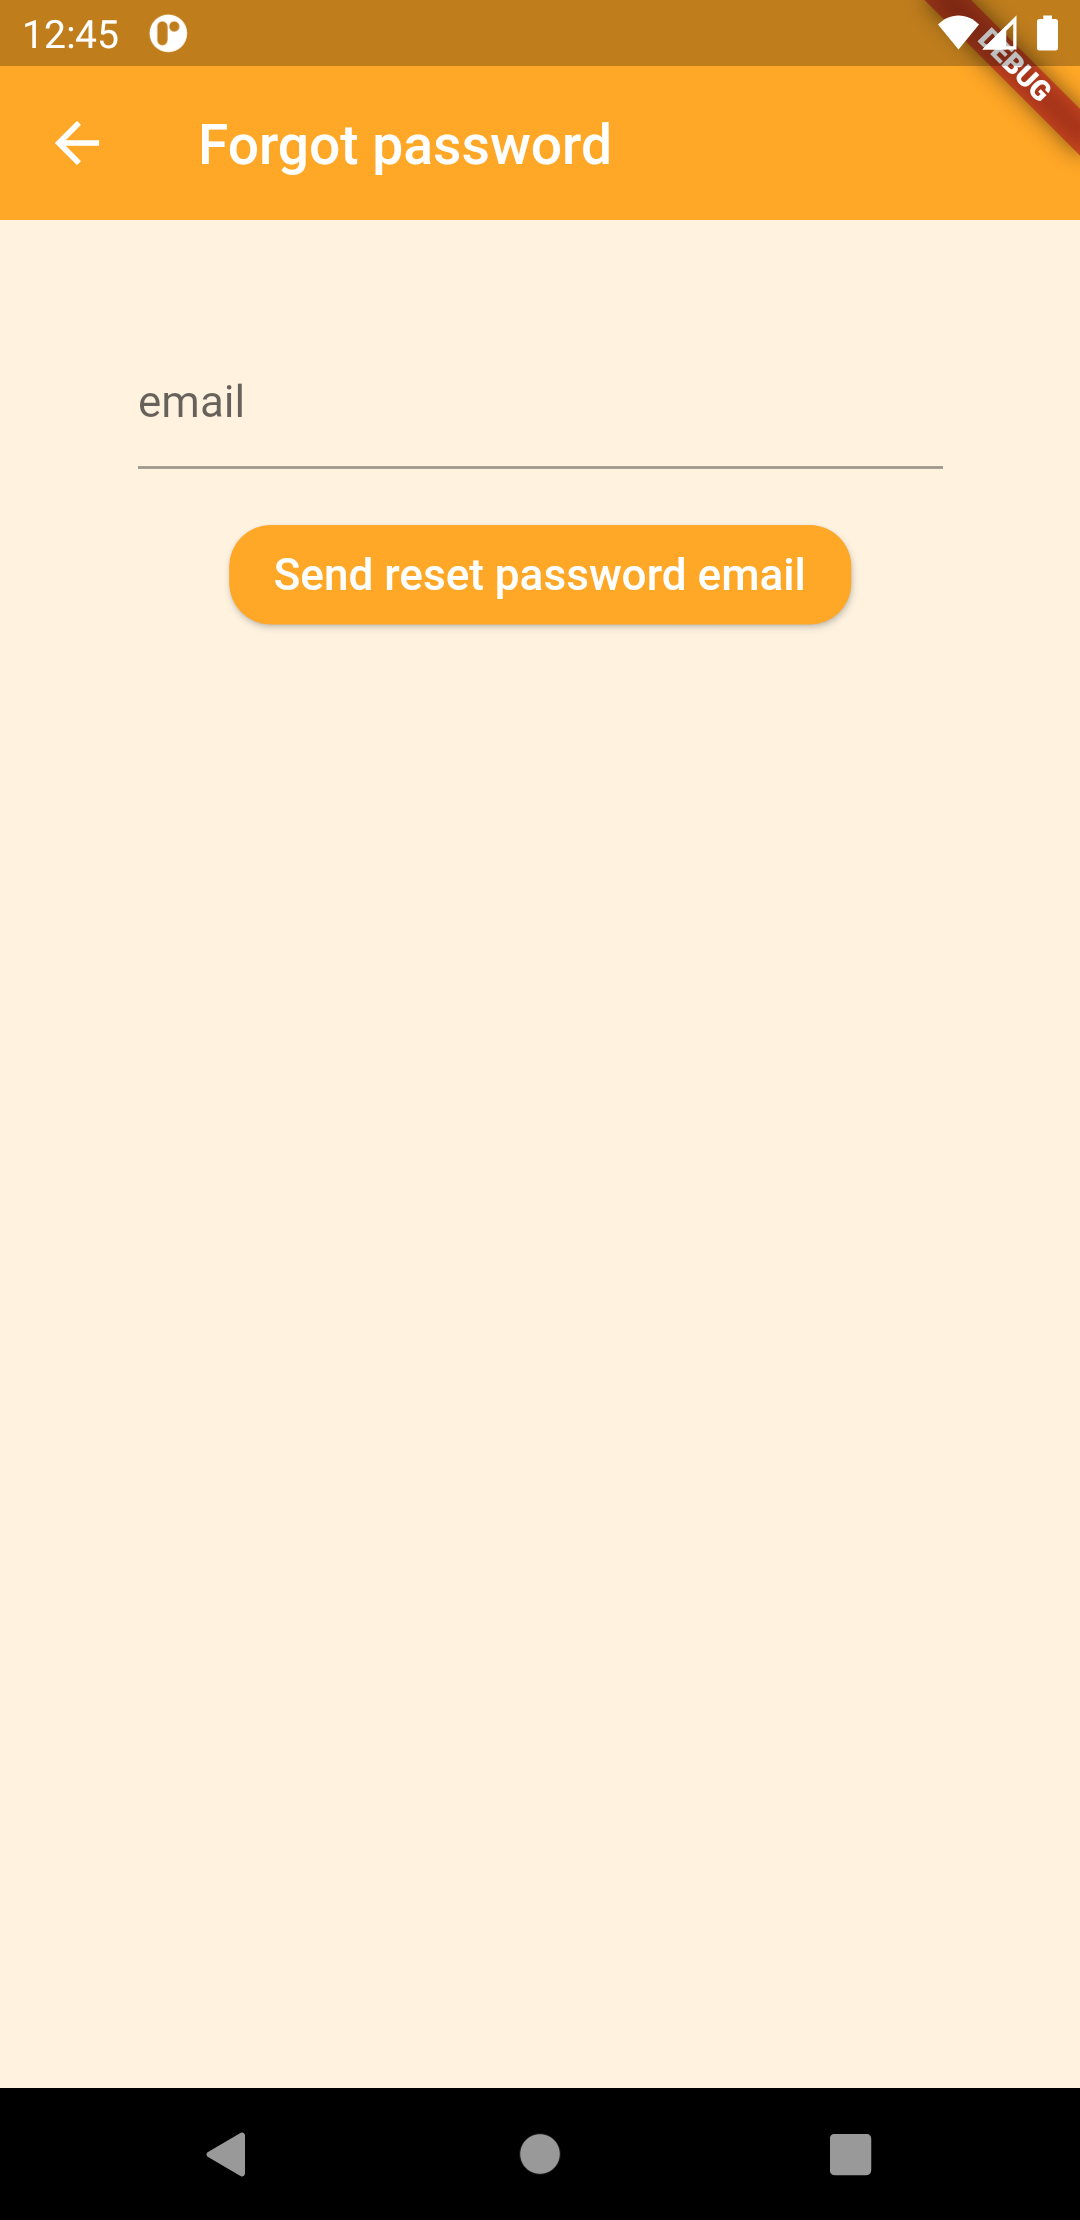
\includegraphics[width = .3\linewidth]{img/PasswordReset.png}
	\caption{Password Reset Screen}
\end{figure}
From this screen the user has the possibility to restore his lost password, providing the email by which he made the registration before.

\subsection{Home}
%TODO image
This is the main screen of the application, from here the user is able to navigate to all the available screens and features of the application by using the navigation bar at the bottom.
It retrieves the ten most recent uploaded recipes and if he keeps scrolling more recipes are shown.

\subsection{Recipe Description}
\begin{figure}[H]
	\begin{minipage}{0.48\textwidth}
		\centering
		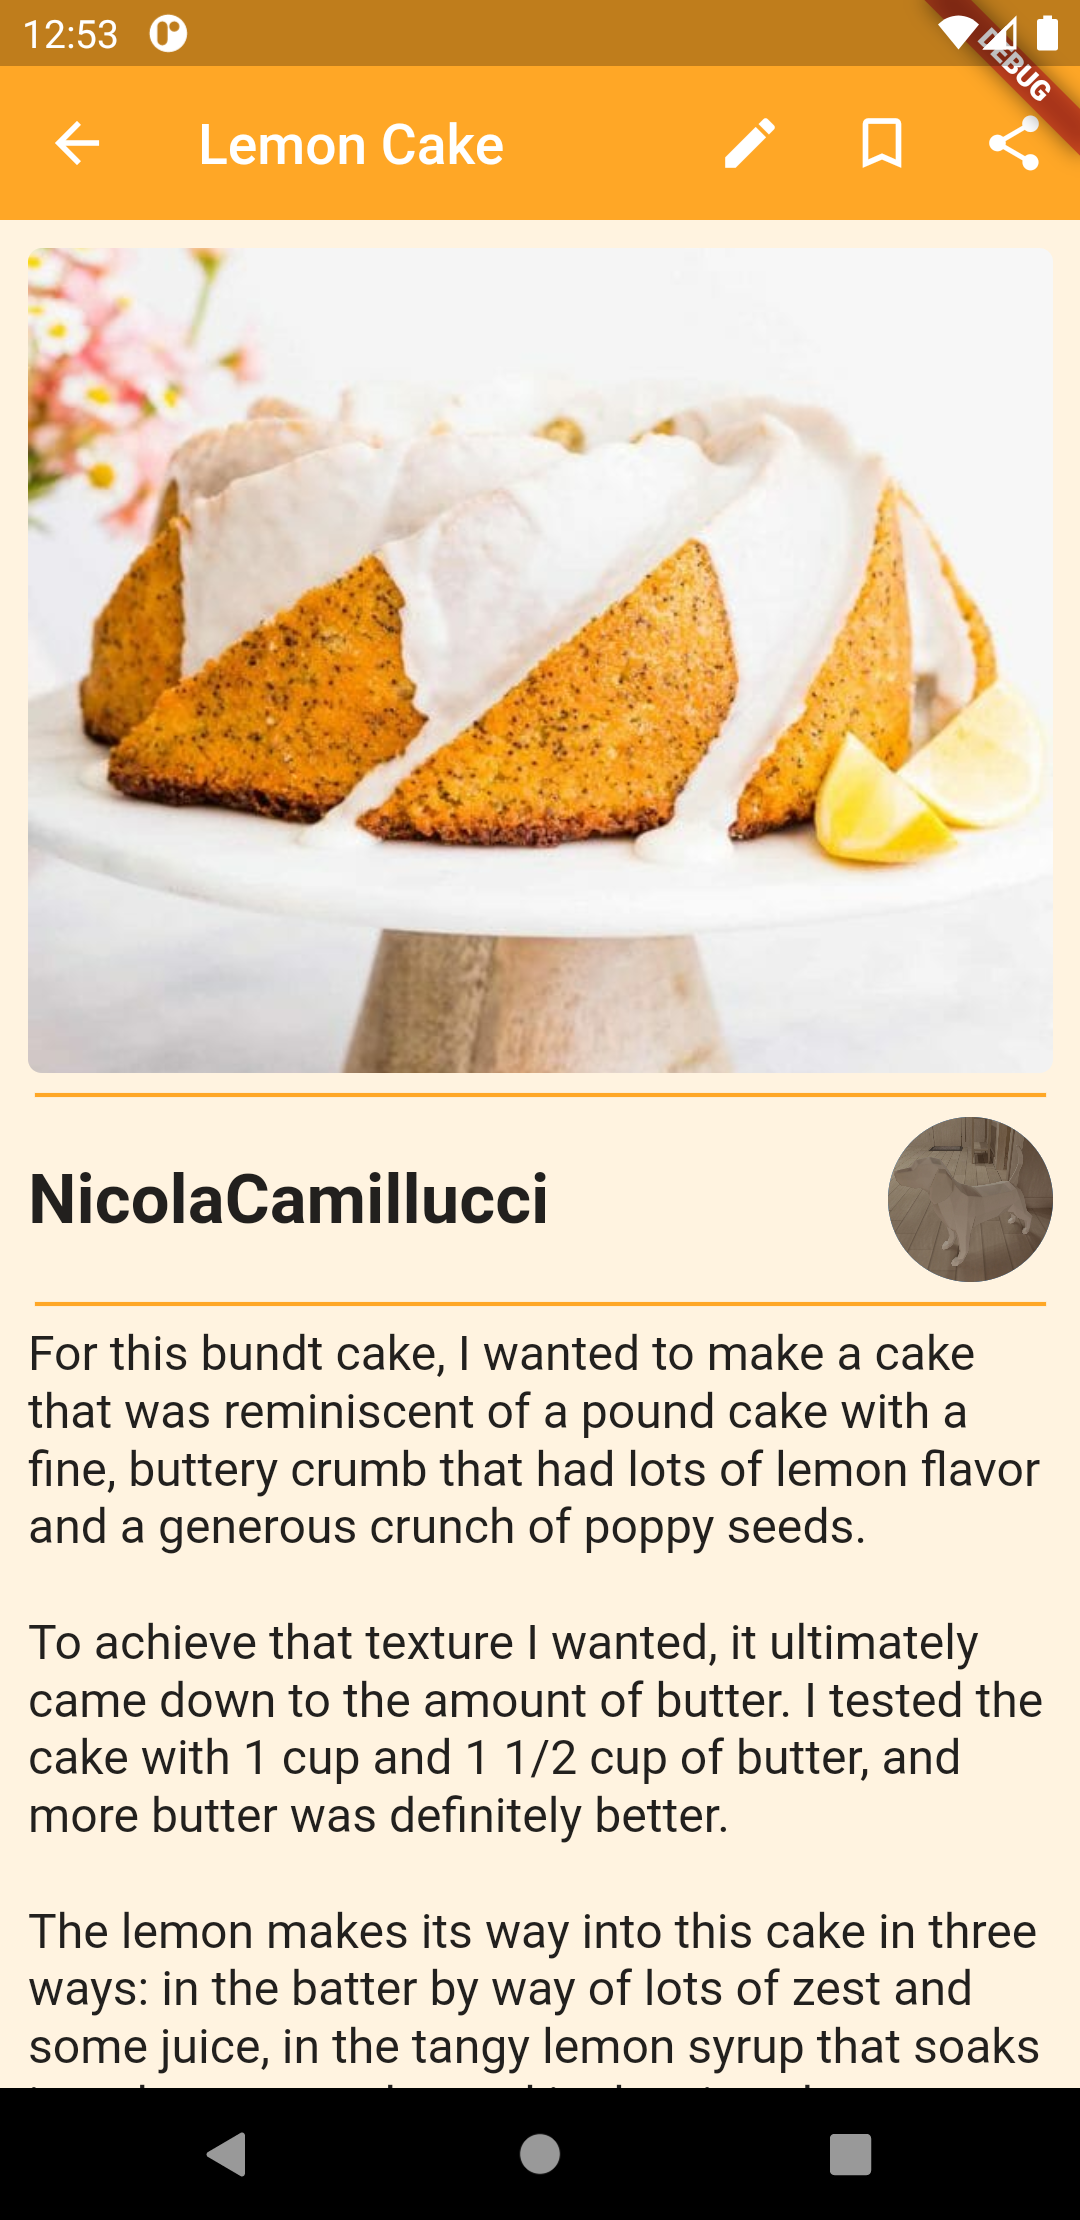
\includegraphics[width = .7\linewidth]{img/RecipeView.png}
		\caption{Recipe View 1 Screen}
	\end{minipage}\hfill
	\begin{minipage}{0.48\textwidth}
		\centering
		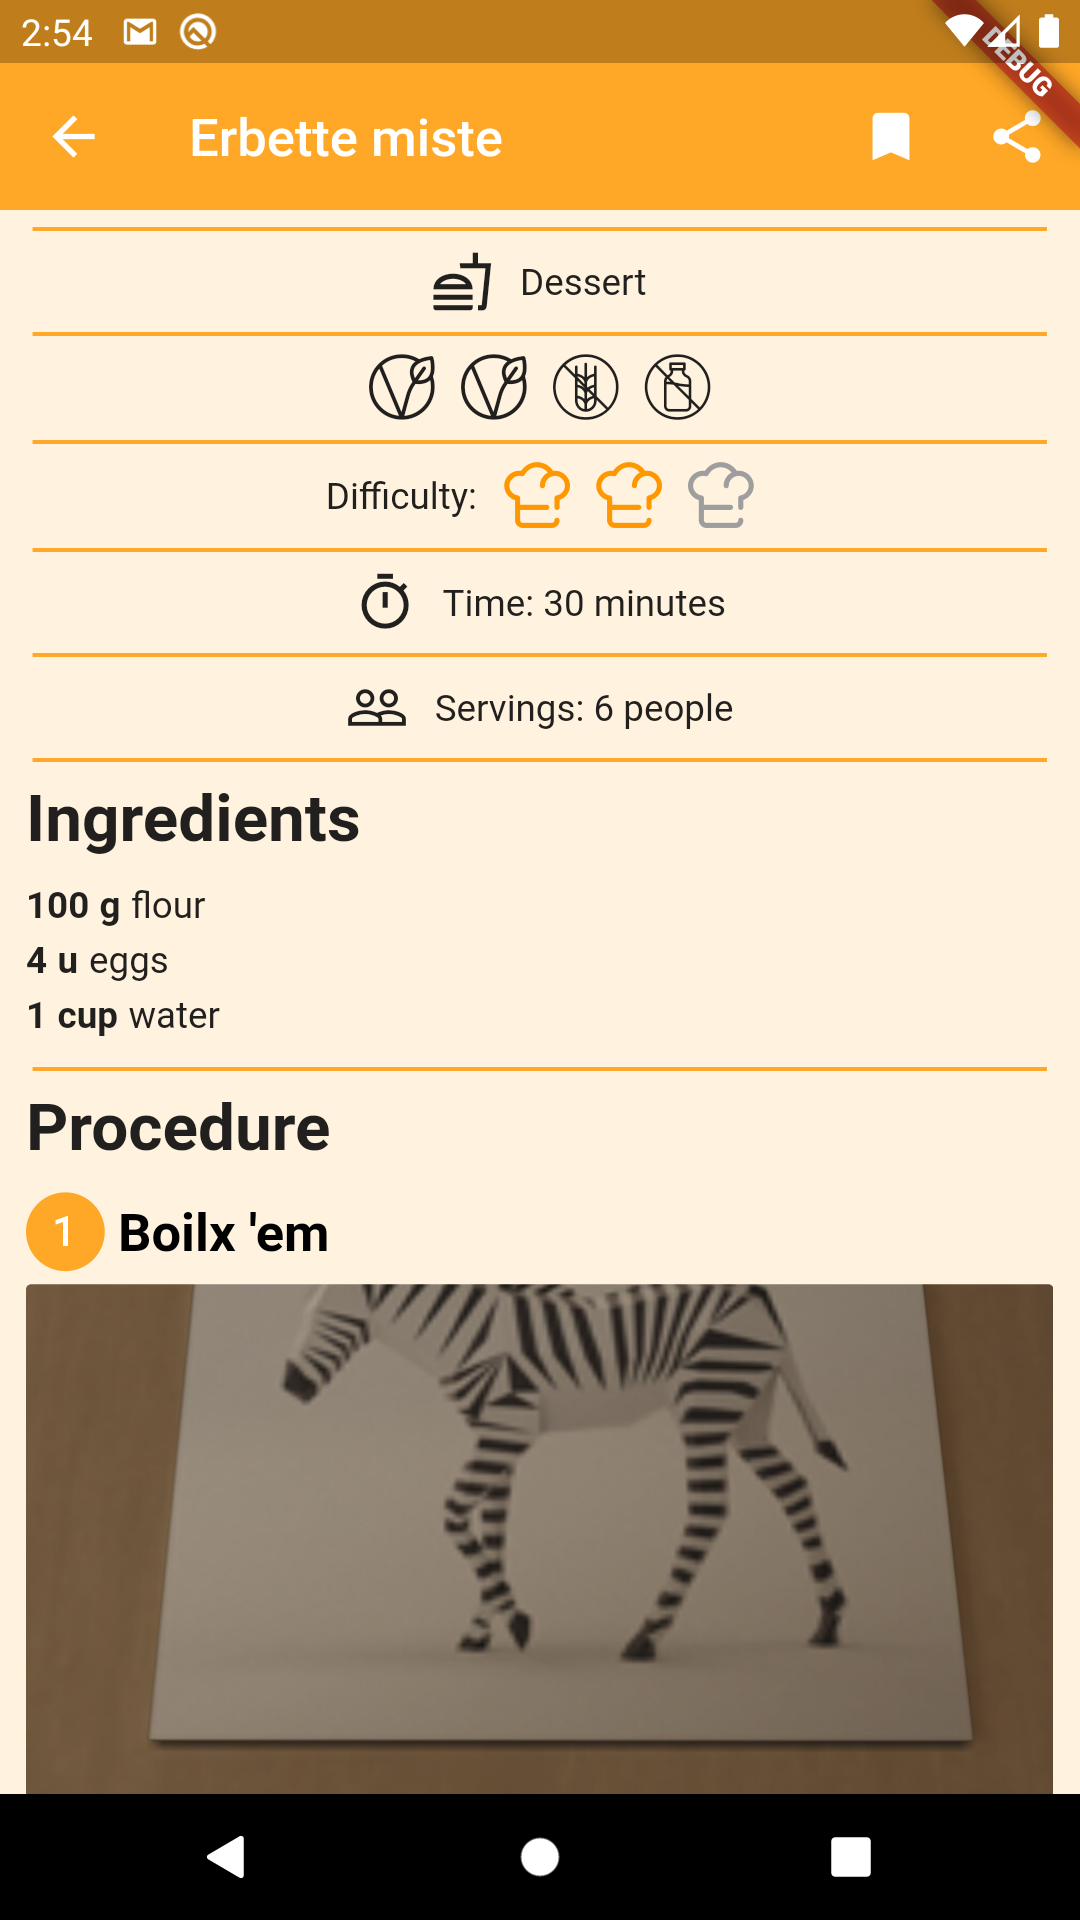
\includegraphics[width = .7\linewidth]{img/RecipeView_2.png}
		\caption{Recipe View 2 Screen}
	\end{minipage}
\end{figure}
This is the screen which appears after clicking on a recipe card.
In the first part it shows the picture of the dish, the author, category, intolerances, difficulty, average preparation time and suggested number of serving.
Then it shows the list of required ingredients and all the procedure to cook the recipe.
At the bottom of this view there is also the list of reviews left by other users, if any.

\subsection{Write a Recipe}
\begin{figure}[H]
	\begin{minipage}{0.31\textwidth}
		\centering
		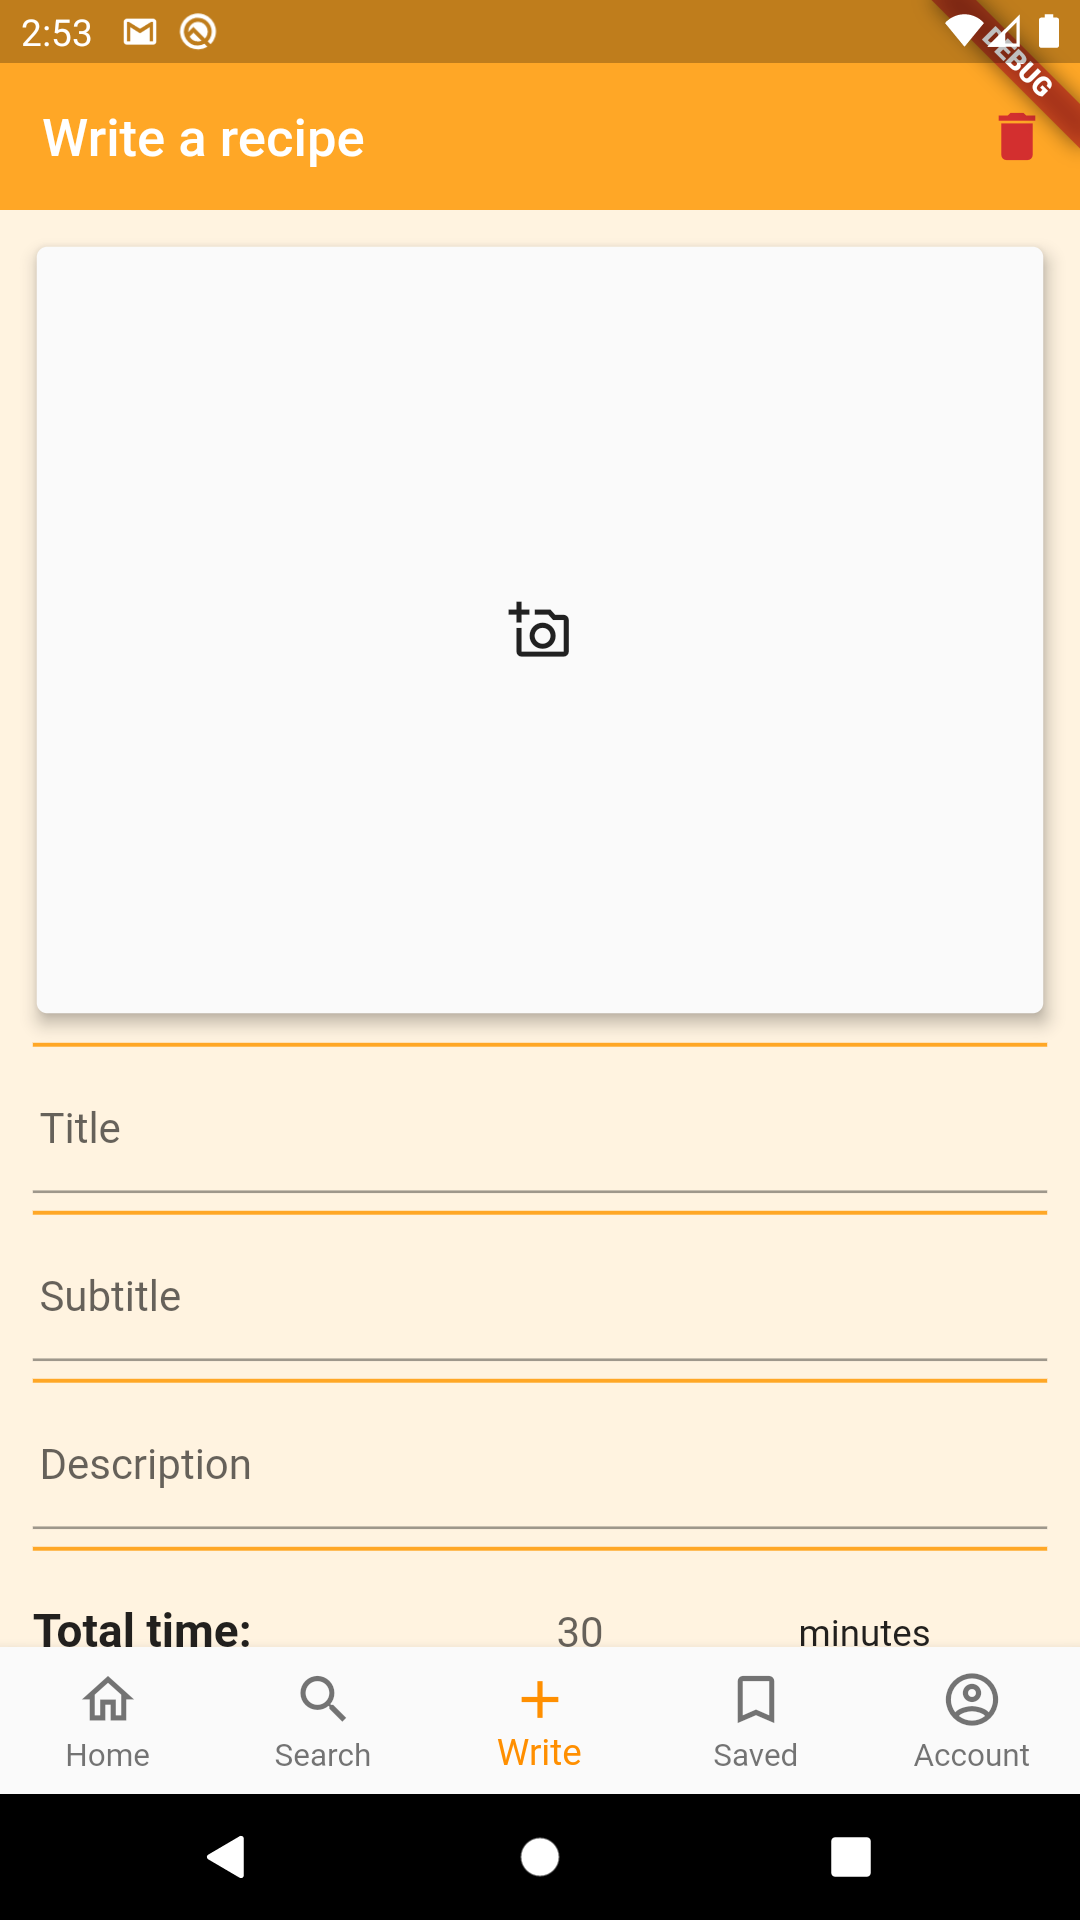
\includegraphics[width = .9\linewidth]{img/Write_1.png}
		\caption{Write Recipe 1 Screen}
	\end{minipage}\hfill
	\begin{minipage}{0.31\textwidth}
		\centering
		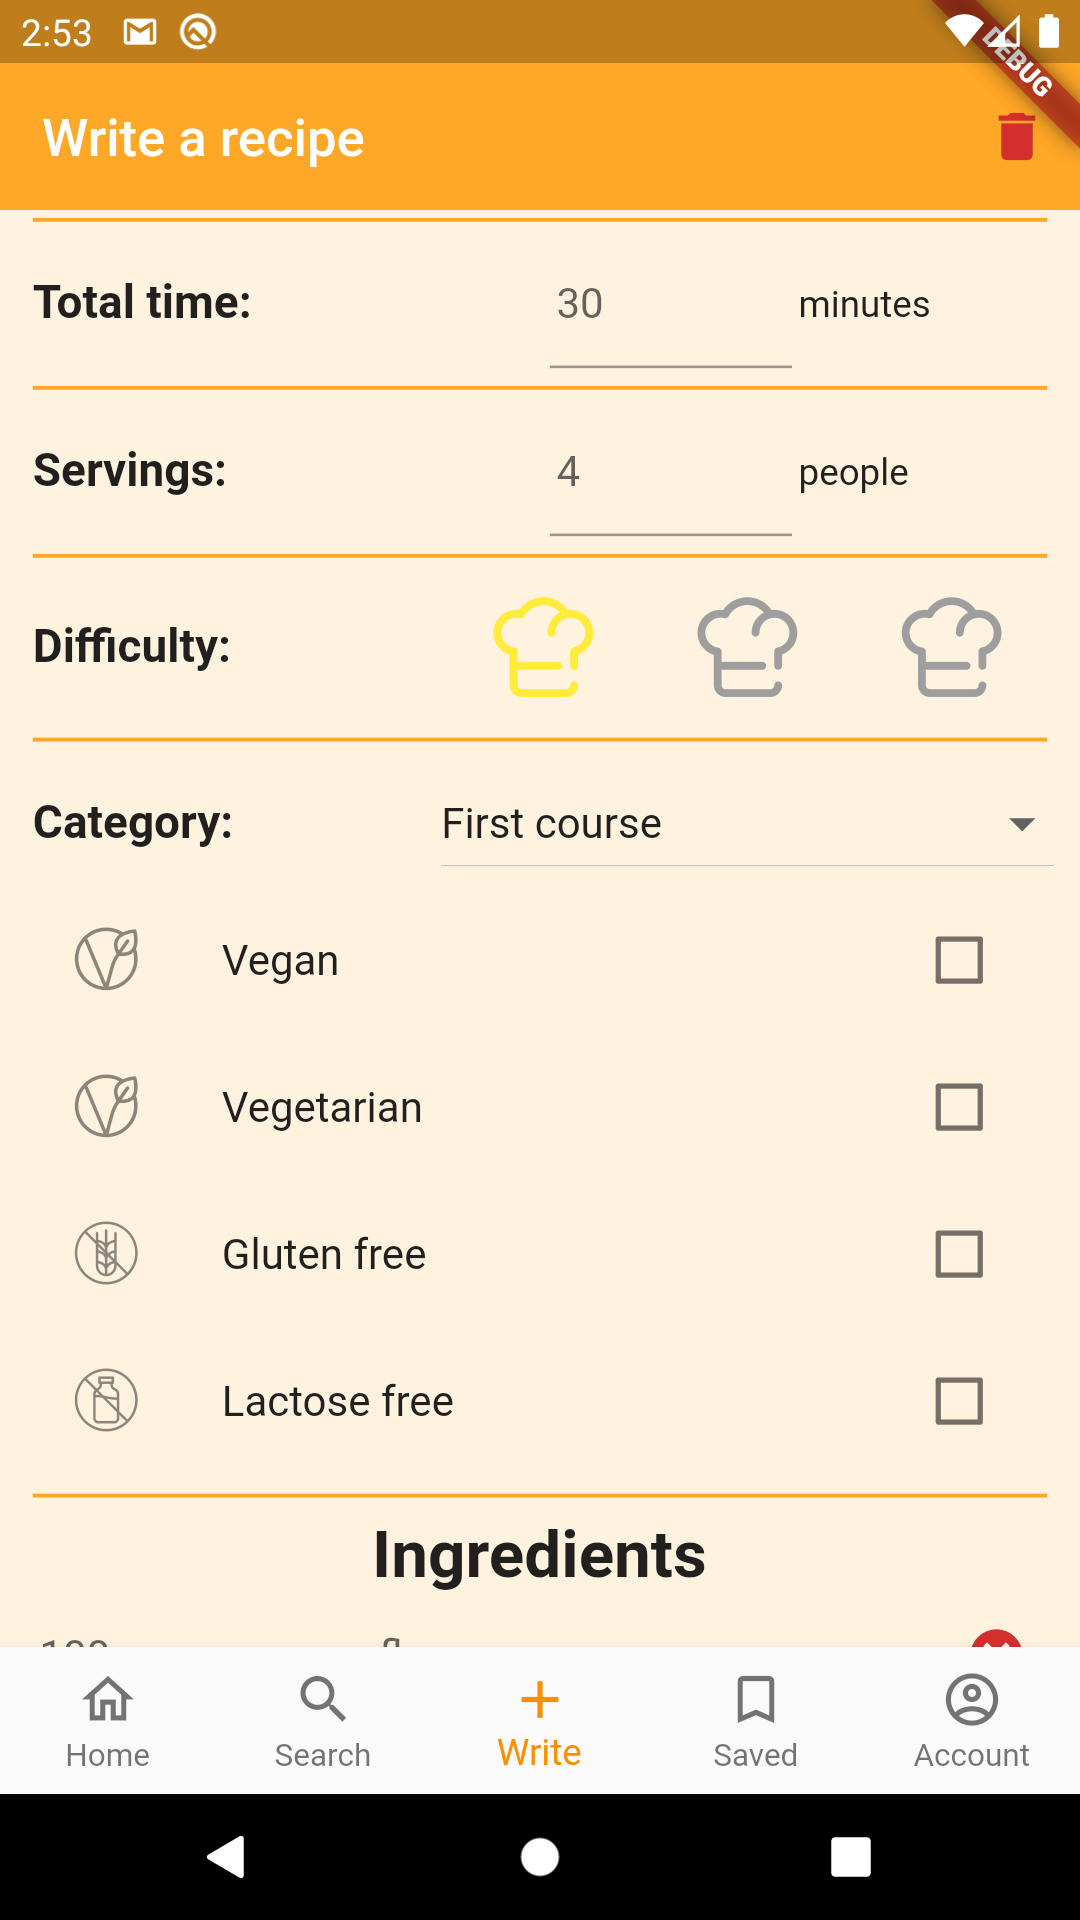
\includegraphics[width = .9\linewidth]{img/Write_2.png}
		\caption{Write Recipe 2 Screen}
	\end{minipage}\hfill
	\begin{minipage}{0.31\textwidth}
		\centering
		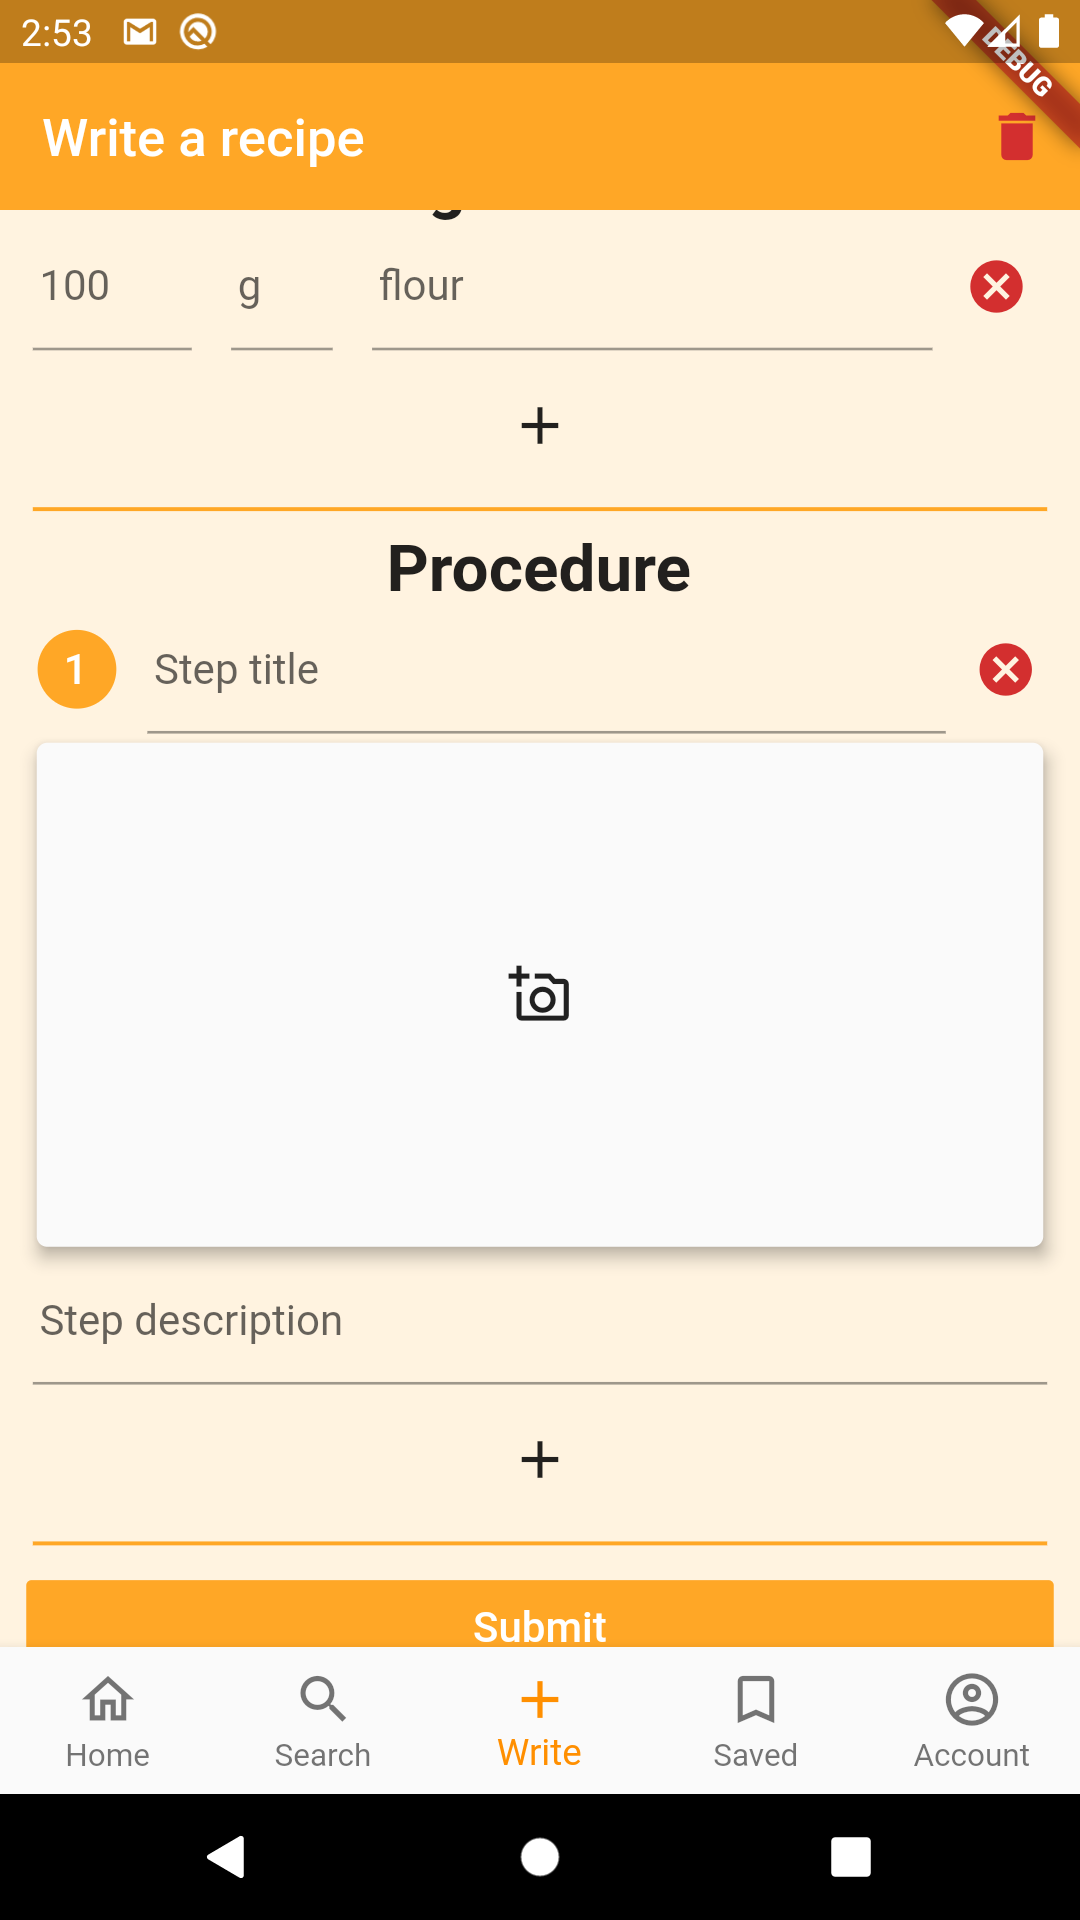
\includegraphics[width = .9\linewidth]{img/Write_3.png}
		\caption{Write Recipe 3 Screen}
	\end{minipage}
\end{figure}
This is the screen used in order to insert a new recipe, which it's reachable from the home page.
Here the user can provide the name of the recipe, the picture of the dish, some information like preparation time, suggested number of serving and intolerances, and especially the ingredients and procedure steps.

\subsection{Search Recipes}
\begin{figure}[H]
	\centering
	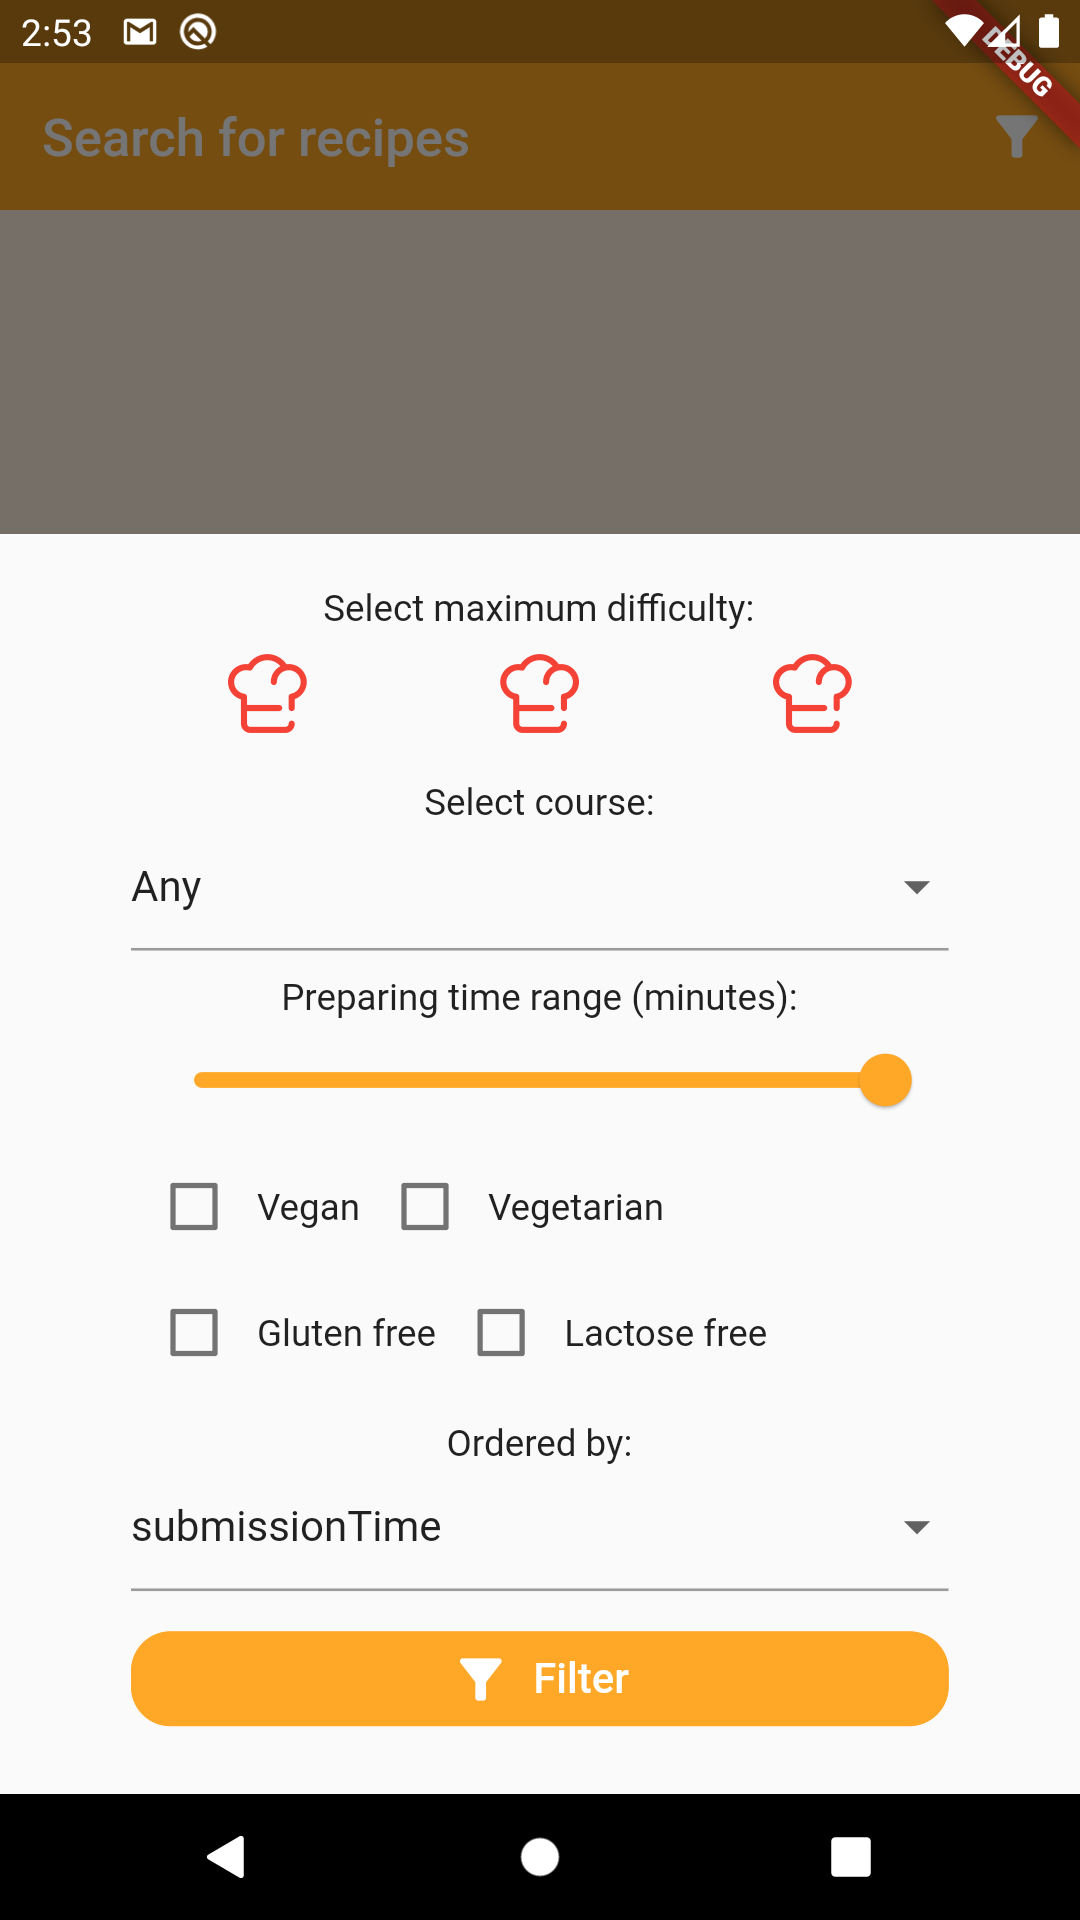
\includegraphics[width = .3\linewidth]{img/Filter.png}
	\caption{Search Recipe Screen}
\end{figure}
This screen, reachable from the home one, gives the possibility to filter the whole database of recipes according to some parameter like duration, difficulty, characteristics...

\subsection{Write a Review}
\begin{figure}[H]
	\centering
	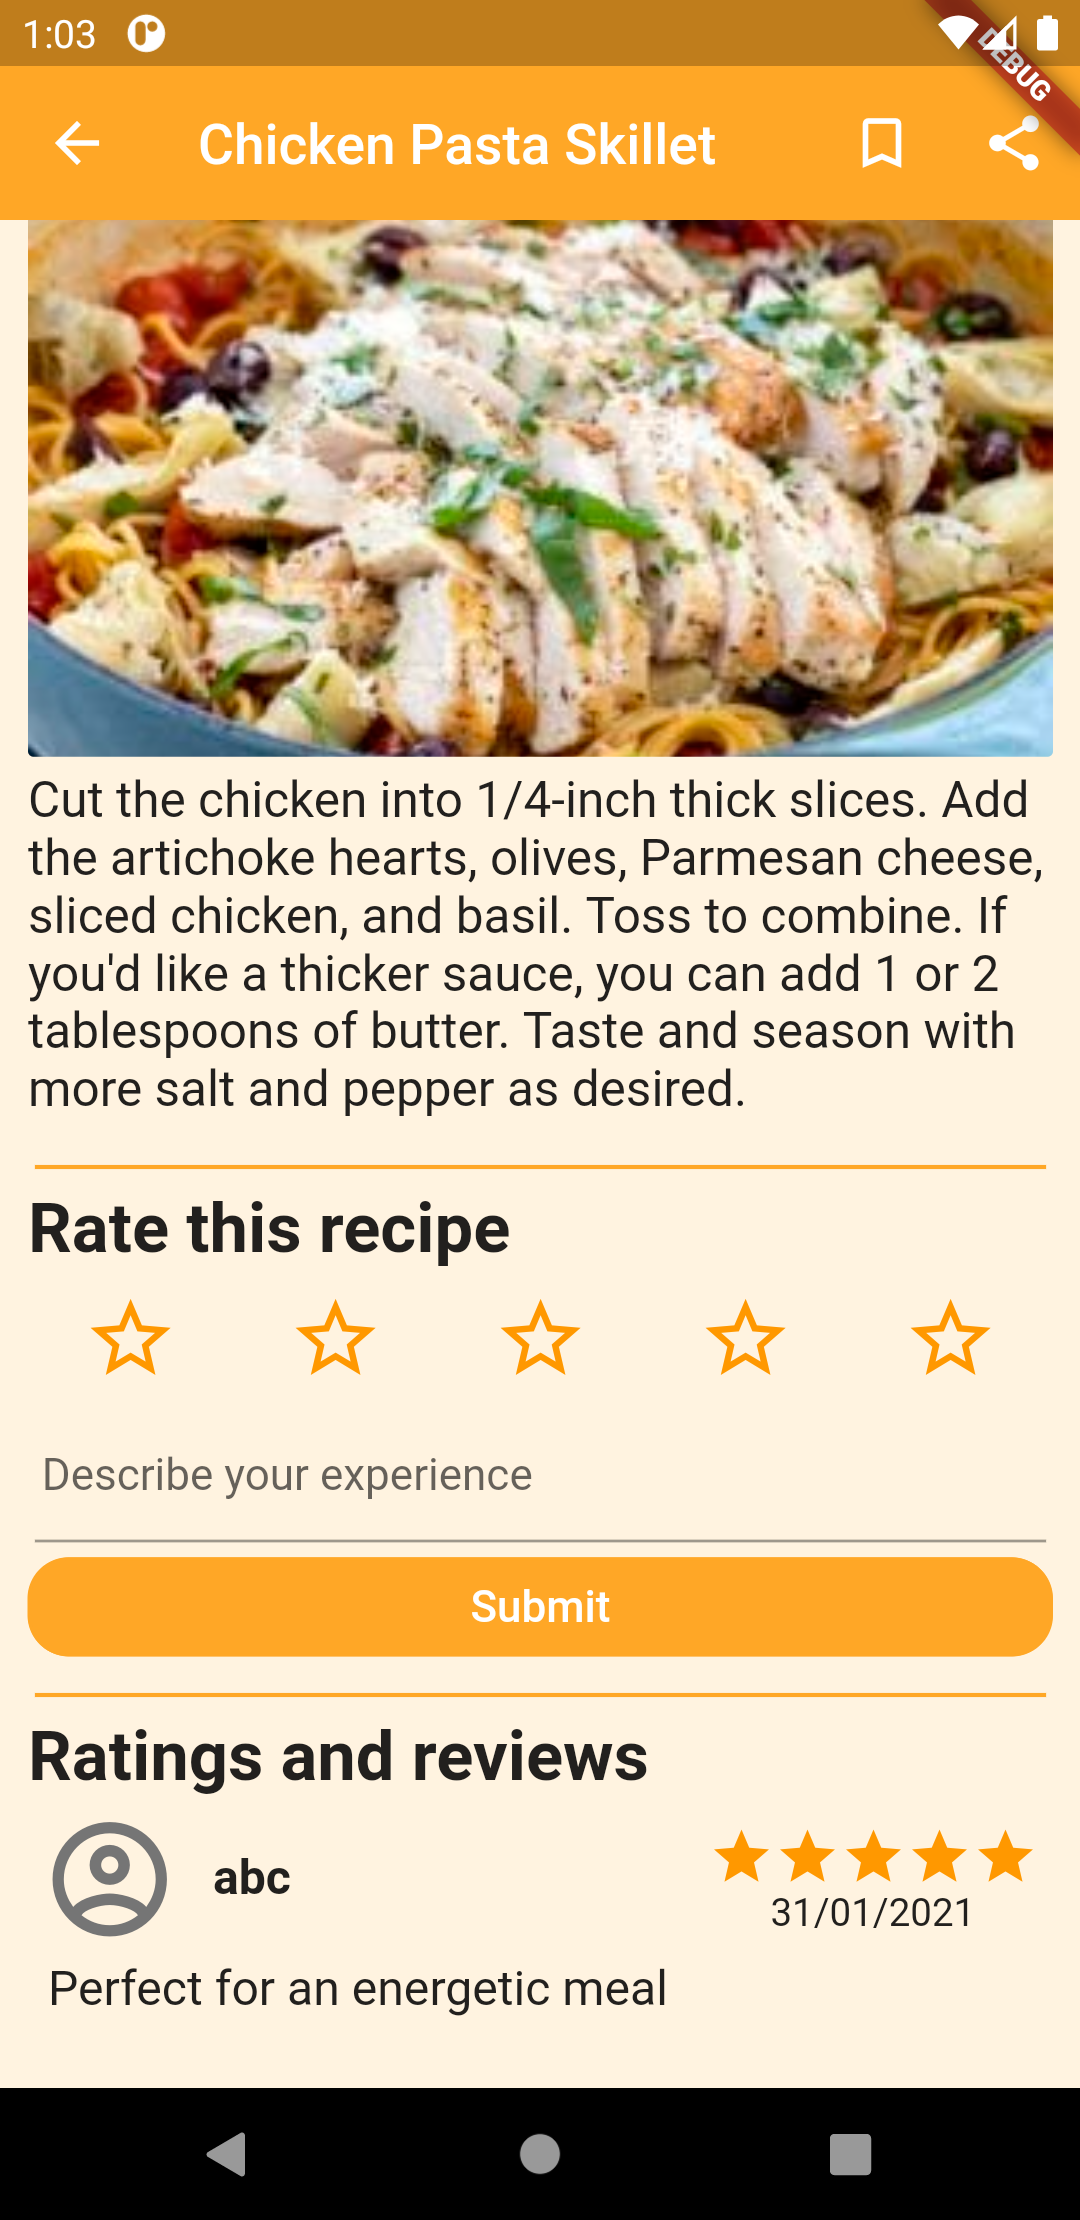
\includegraphics[width = .3\linewidth]{img/Review.png}
	\caption{Review Screen}
\end{figure}
This screen allows the user to leave a review for the visualized recipe, by giving a rating and adding a comment.
The review can also be deleted afterwards.

\subsection{Saved Recipes}
\begin{figure}[H]
	\centering
	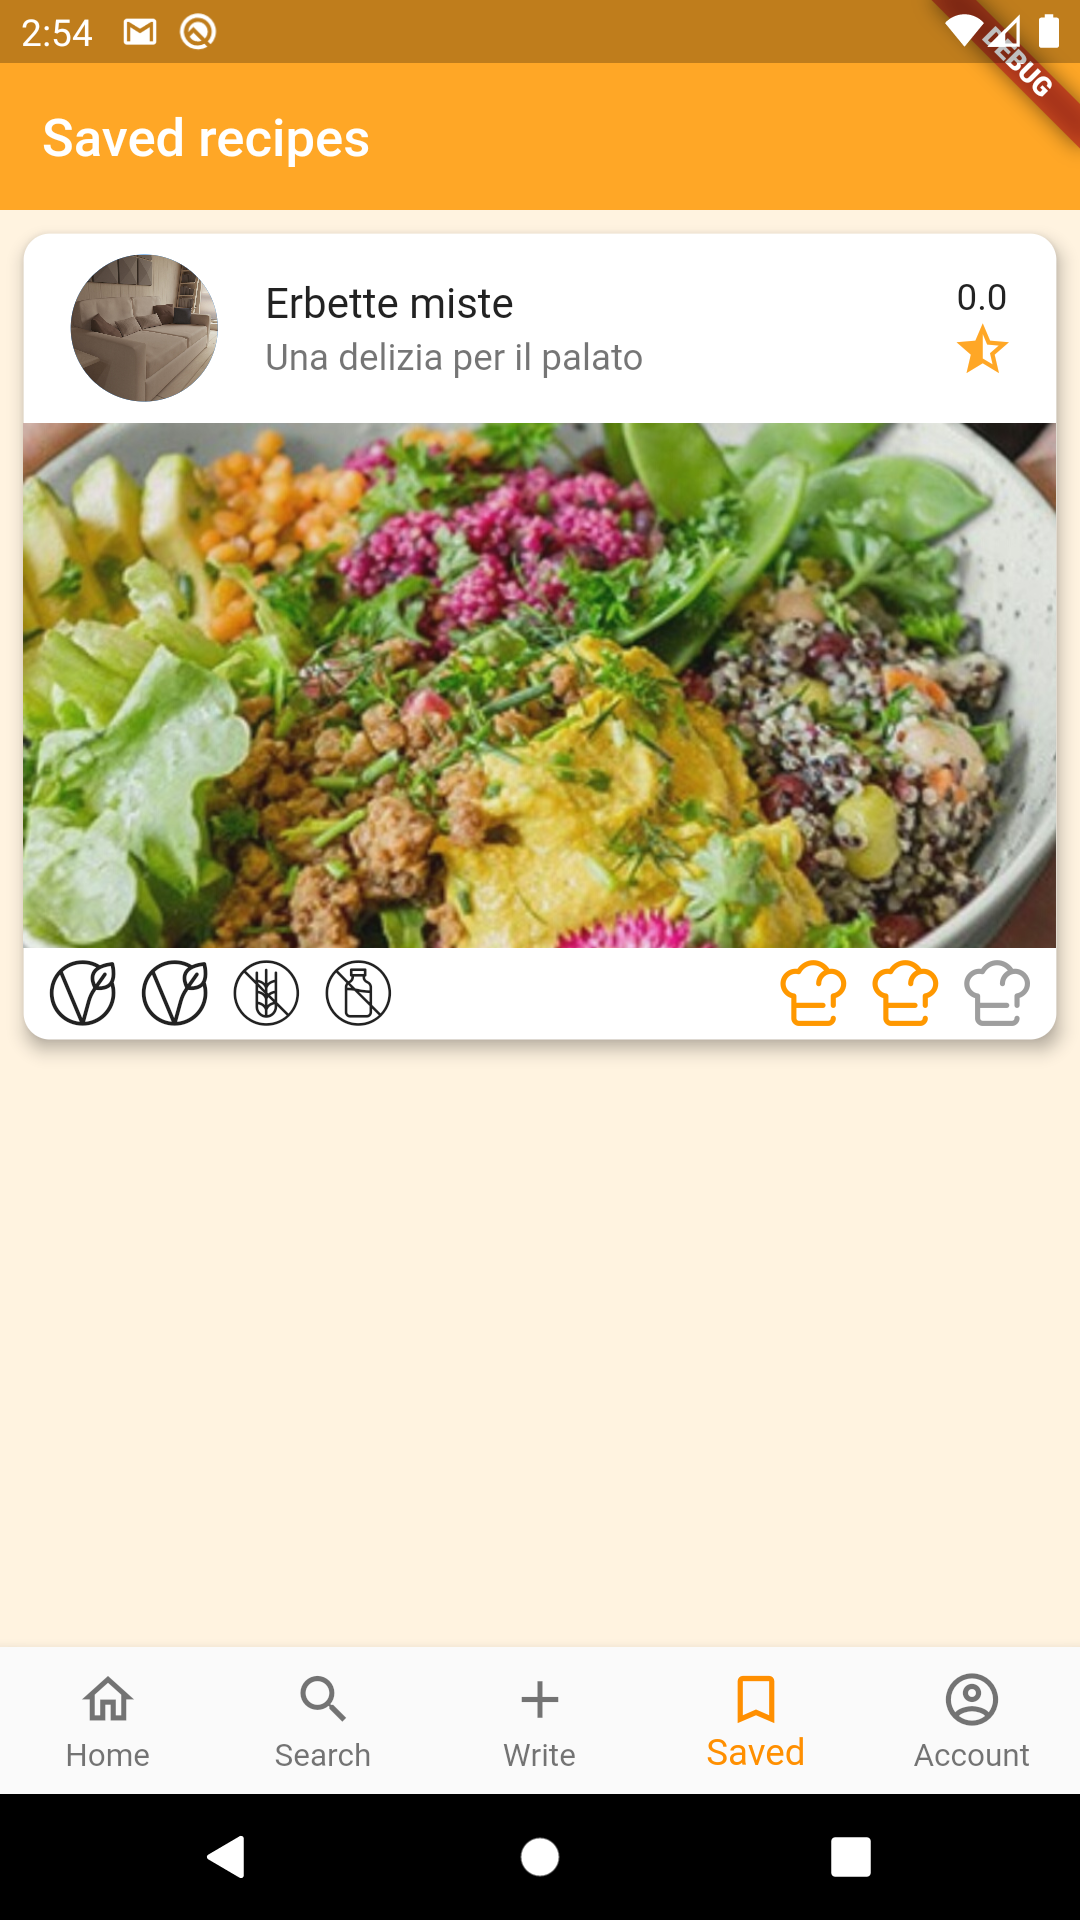
\includegraphics[width = .3\linewidth]{img/Saved.png}
	\caption{Saved Recipe Screen}
\end{figure}
This screen is accessible from the home screen and it lists all the recipes saved by the user displayed in random order.

\subsection{User Profile}
%TODO image
This screen shows the user profile statistics, which are number of written recipes, number of received reviews and average rating, and the list of the user uploaded recipes.
From here the user can also perform the log out from his/her account.

\subsection{Settings}
%TODO image
This screen allows the user to modify his profile picture, username and the password (only if he is logged using the email).
